\documentclass[11pt,a4paper]{book}
\usepackage[utf8]{inputenc}
\usepackage[T1]{fontenc}
\usepackage[italian]{babel}
\usepackage{lmodern}
\usepackage{amsmath,amssymb}
\usepackage{graphicx}
\usepackage{float}
\usepackage{hyperref}
\usepackage{booktabs}
\usepackage{longtable}
\usepackage{array}
\usepackage{caption}
\graphicspath{{images/}}

\title{Fisica Tecnica}
\author{}
\date{\today}

\begin{document}
\maketitle
\tableofcontents


\chapter{2 - Introduzione}
\input{chapters/01-2-introduzione.tex}

\chapter{3 - Energia}
\input{chapters/02-3-energia.tex}

\chapter{4 - Proprietà delle sostanze pure}
Una sostanza pura è una sostanza in cui la composizione chimica non
varia in tutta la massa considerata. \#\#\# Fasi di una sostanza pura
Una sostanza pura si può trovare in 3 fasi: - Solida - Liquida - Gassosa

Un liquido può essere \textbf{sottoraffreddato} (non in procinto di
evaporare) o \textbf{saturo} (in procinto di evaporare). Analogamente un
vapore \textbf{saturo} è in procinto di condensare e uno
\textbf{surriscaldato} no. Tra un liquido saturo e un vapore saturo c'è
la \textbf{miscela satura di liquido e vapore}.
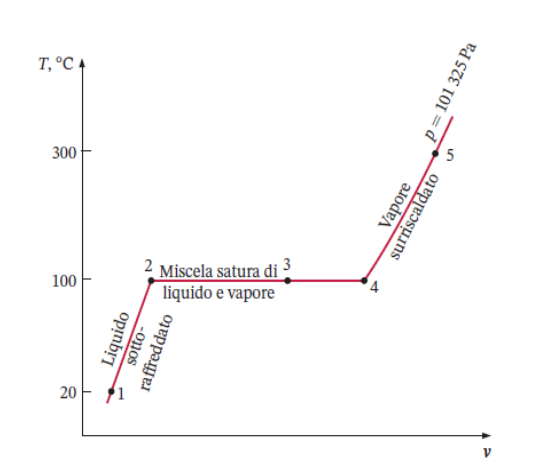
\includegraphics{Fasi.png}

\emph{Diagramma di un processo di riscaldamento dell'acqua a pressione
costante}

\hypertarget{proprietuxe0}{%
\subsubsection{Proprietà}\label{proprietuxe0}}

\textbf{Temperatura di saturazione} \(T_\text{sat}\): Temperatura a cui
una sostanza inizia a evaporare (fissata la pressione) \textbf{Pressione
di saturazione} \(p_\text{sat}\): Pressione a cui una sostanza inizia a
evaporare (fissata la temperatura) \textbf{Calore latente}: quantità di
energia assorbita (o liberata) durante trasformazione con cambio di fase
\textbf{Calore latente di fusione}: La quantità di energia assorbita
durante la fusione uguale a quella liberata durante solidificazione.
\textbf{Calore latente di vaporizzazione}: La quantità di energia
assorbita durante la vaporizzazione uguale a quella liberata durante la
condensazione. \textbf{Punto critico}: punto in cui coesistono vapore
saturo e liquido saturo. \textbf{Volume specifico} \(v\): reciproco
della densità \textbf{Titolo} \(x\): rapporto tra massa vapore e massa
totale in una miscela. \(x\in[0,1]\), se \(x=0\) liquido saturo, se
\(x=1\) vapore saturo. Un liquido saturo mantiene le proprietà anche
quando è in una miscela con vapore.

\hypertarget{entalpia}{%
\subsubsection{Entalpia}\label{entalpia}}

\(h=u+pv\hspace{0.4cm}(kJ/kg)\) \(H=U+pV\hspace{0.4cm}(kJ)\) Entalpia di
vaporizzazione \(h_\text{l,sat}\) (calore latente di vaporizzazione):
Energia necessaria a trasformare l'unità di massa di un liquido saturo
in vapore saturo a una certa pressione e temperatura.


\chapter{5 - Analisi energetica dei sistemi chiusi}
\input{chapters/04-5-analisi-energetica-dei-sistemi-chiusi.tex}

\chapter{6 - Analisi dei volumi di controllo in base alla conservazione della massa e dell’energia}
\input{chapters/05-6-analisi-dei-volumi-di-controllo-in-base-alla-conservazione-della-massa-e-dellenergia.tex}

\chapter{8 - Entropia}
\input{chapters/06-8-entropia.tex}

\chapter{12 - Le modalità di trasmissione del calore}
\input{chapters/07-12-le-modalita-di-trasmissione-del-calore.tex}

\chapter{13 - Conduzione}
\input{chapters/08-13-conduzione.tex}

\chapter{15 - Convezione forzata esterna}
\input{chapters/09-15-convezione-forzata-esterna.tex}

\chapter{16 - Convezione forzata interna}
Per flussi in tubi circolari \(L_c=D\) (diametro tubo) Se il tubo non è
circolare \(L_c=D_h=\frac{4A_c}{p}\)


\chapter{17 - Convezione naturale}
\input{chapters/11-17-convezione-naturale.tex}

\chapter{18 - Irraggiamento}
\input{chapters/12-18-irraggiamento.tex}

\chapter{Termodinamica}
\input{chapters/13-termodinamica.tex}

\end{document}
